\part*{Appendix}
\chapter{Models and Figures}
\section{Models}
\label{sec:app-models}

\begin{figure}[H]
	{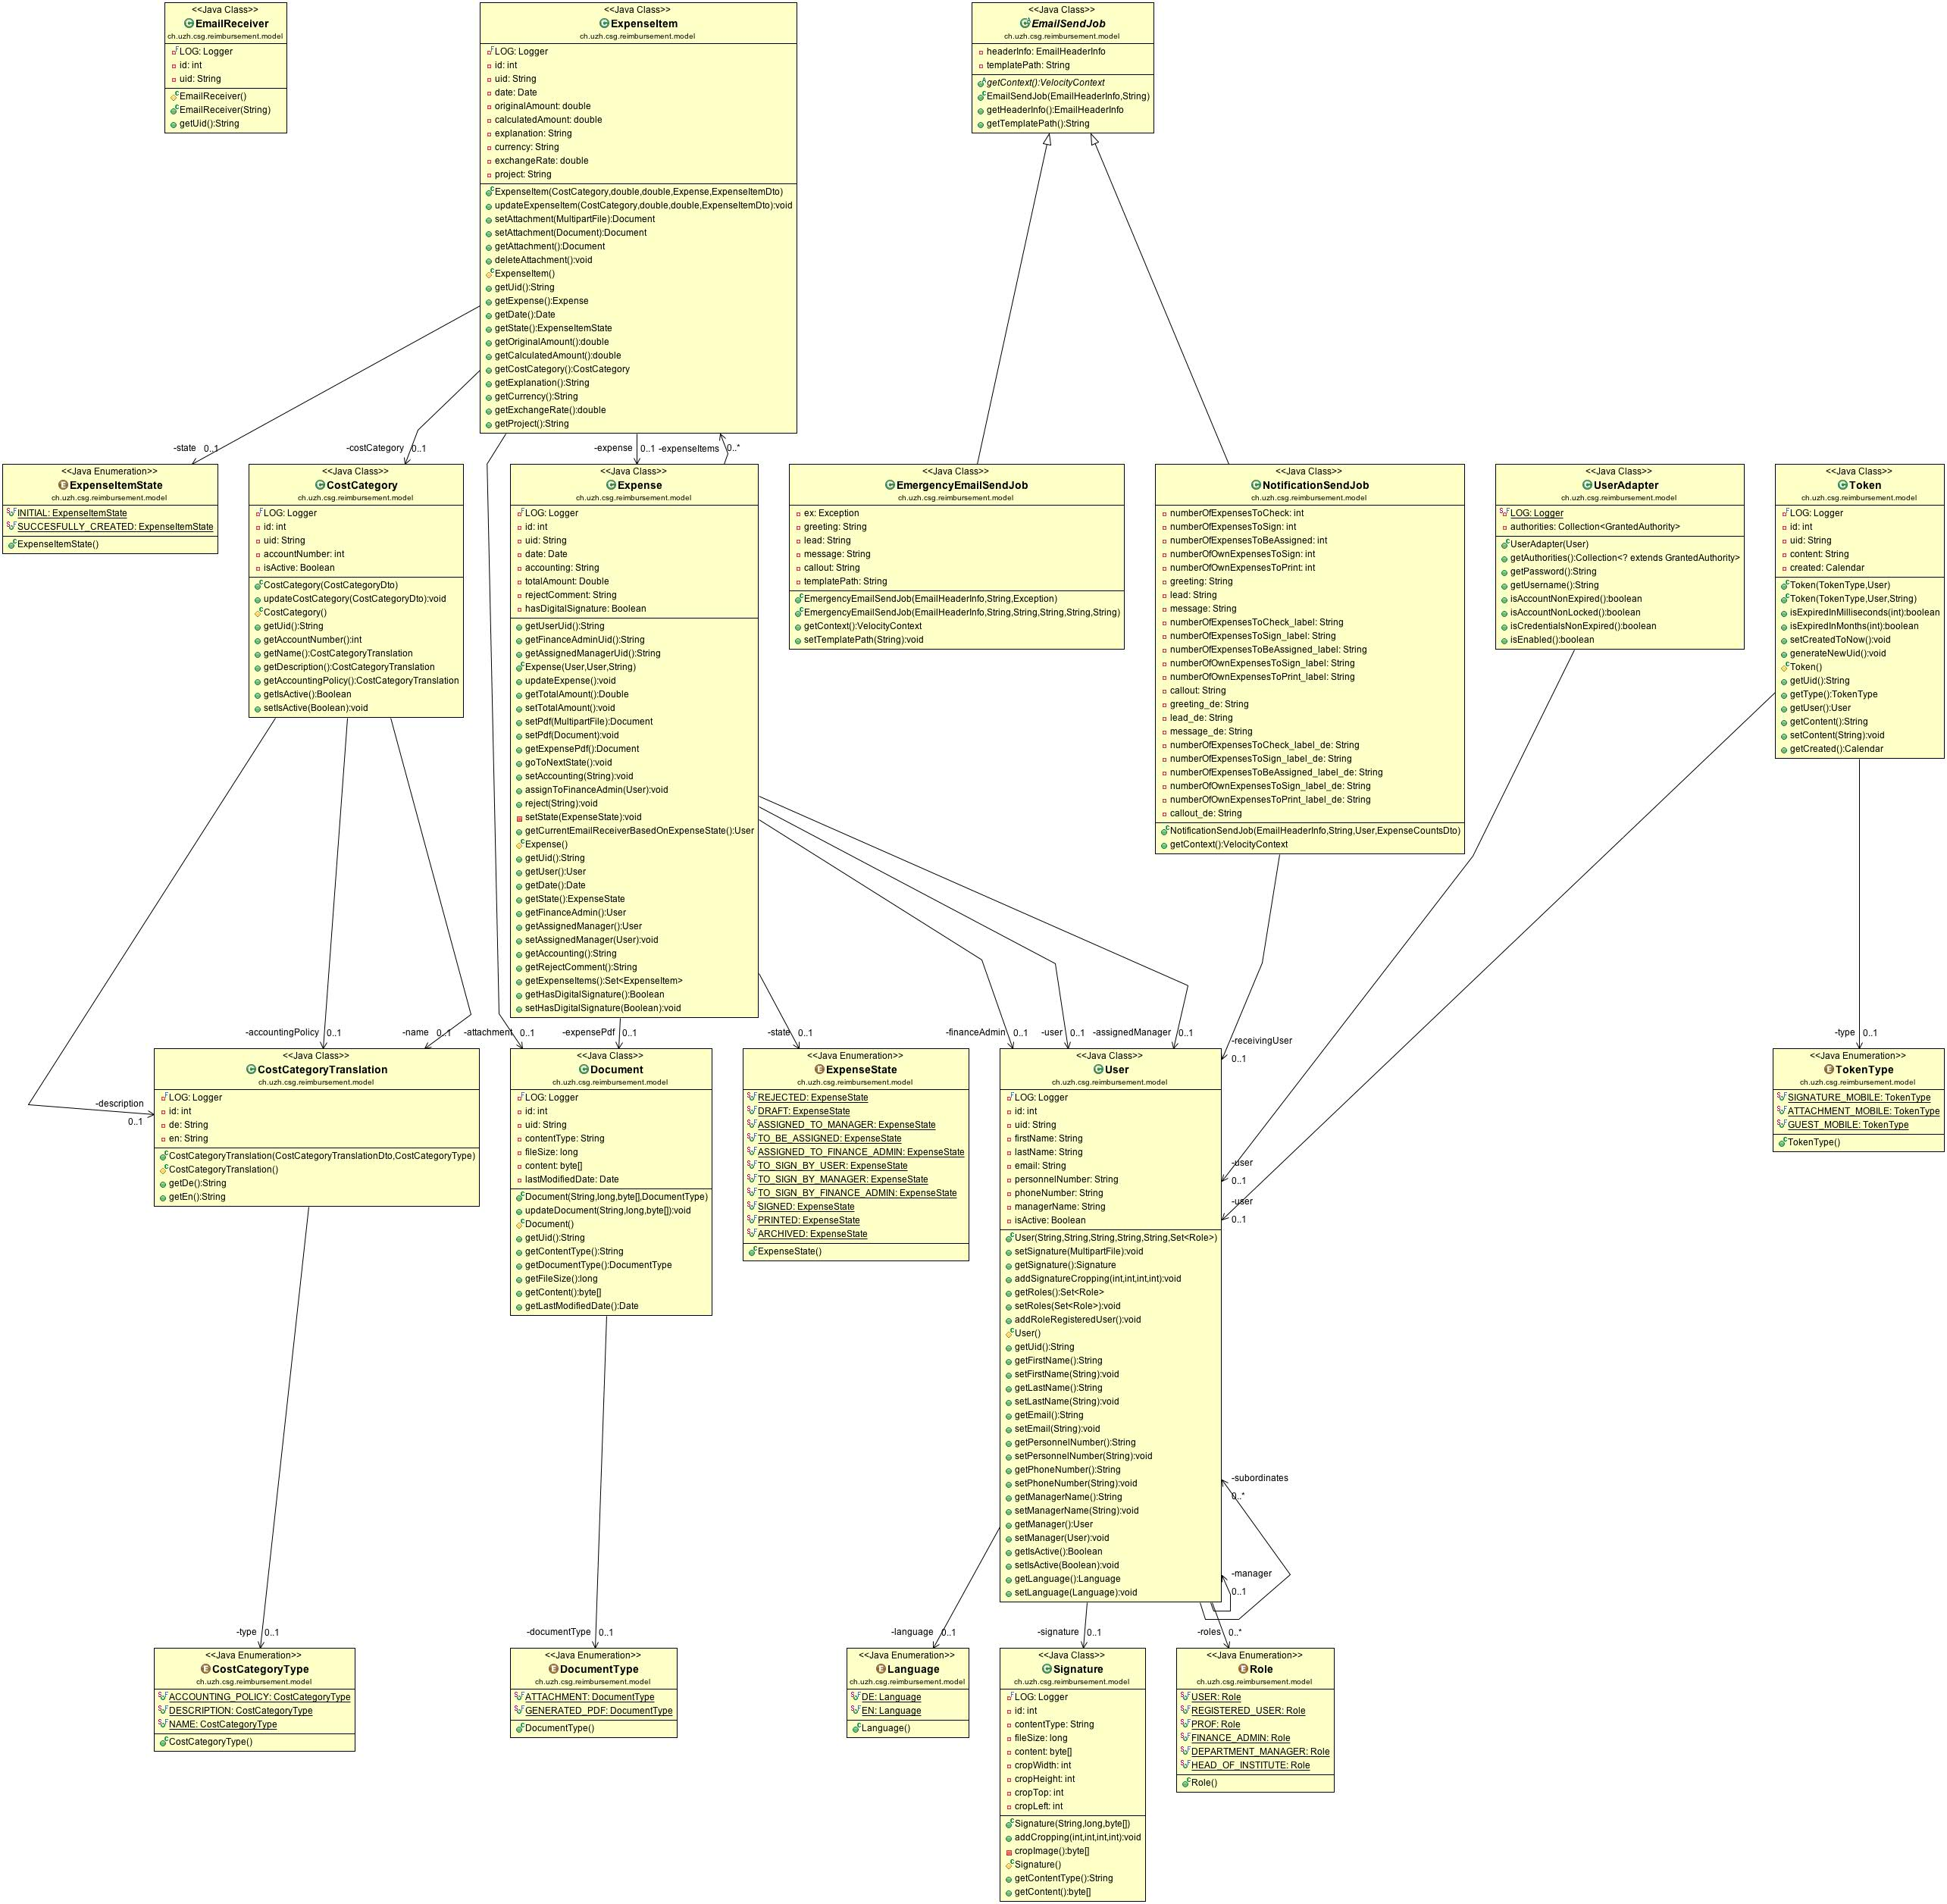
\includegraphics[width=1.0\textwidth]{umlclass-model}}
\end{figure}
\newpage

\section{Services}
\label{sec:app-service}

\begin{figure}[H]
	{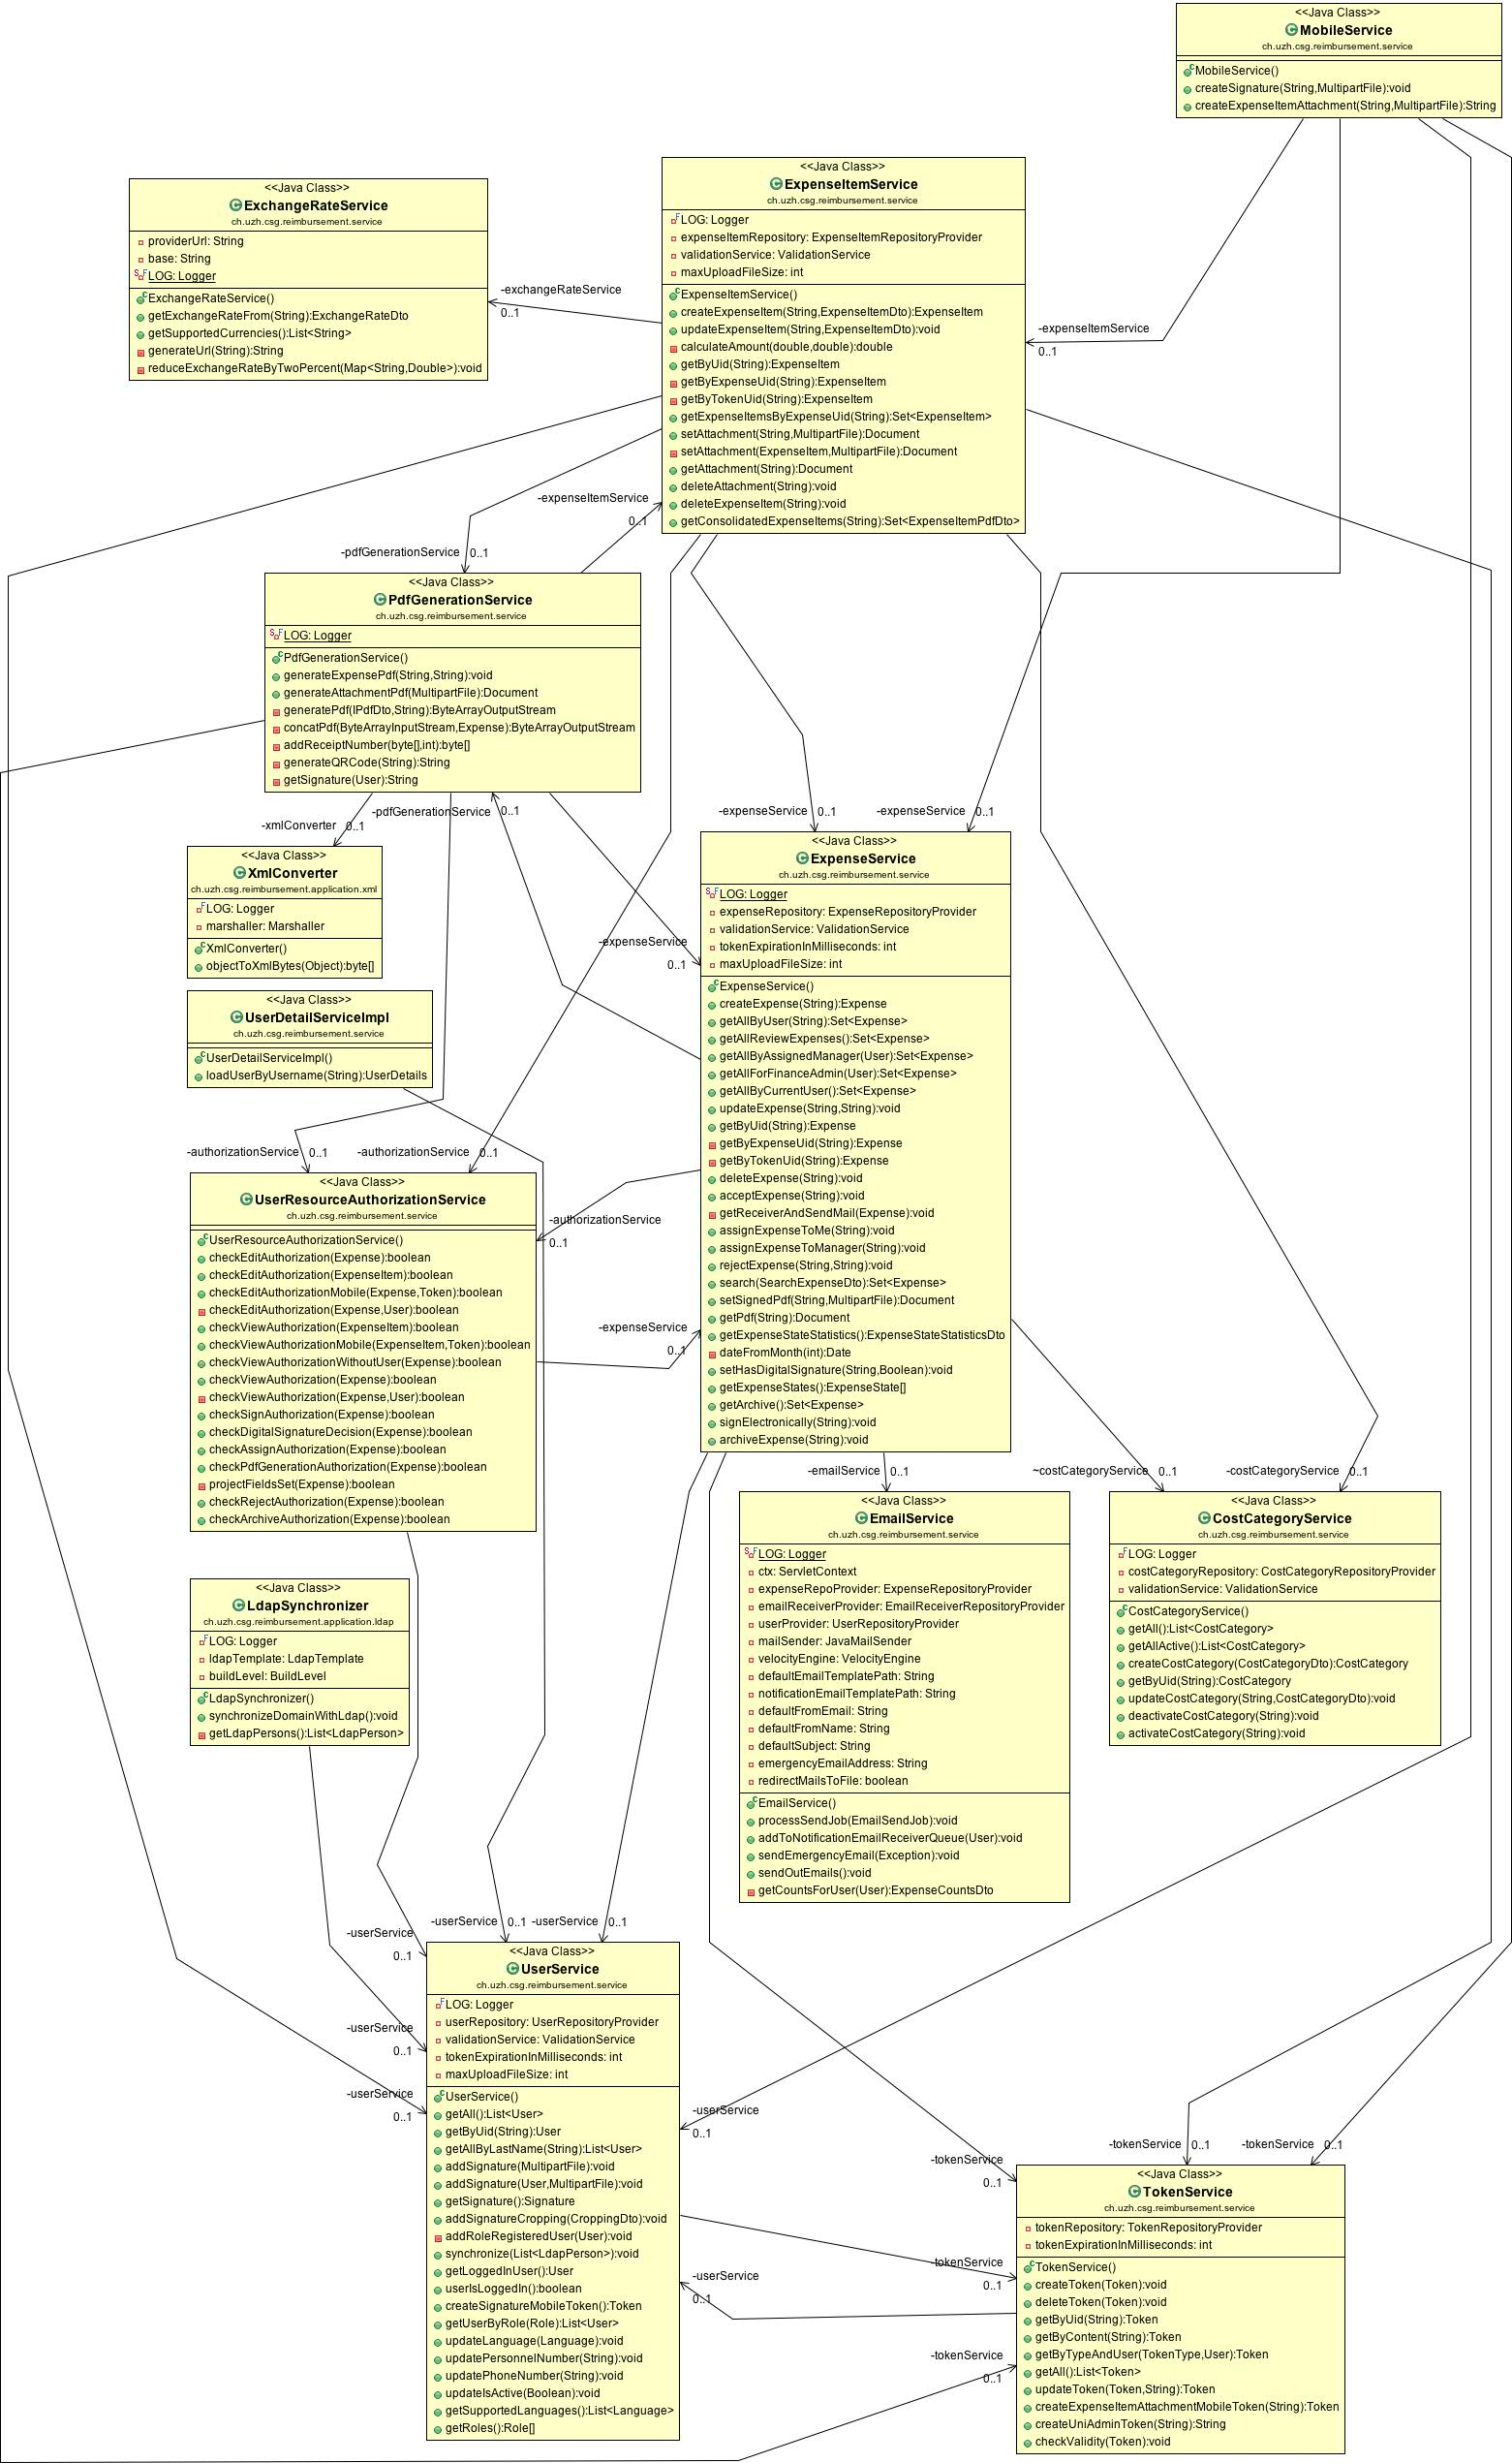
\includegraphics[width=0.8\textwidth]{umlclass-service}}
\end{figure}
\newpage

\section{REST Services}
\label{sec:rest-services}

\subsection{PRIVATE: expense services}
\begin{figure}[H]
	{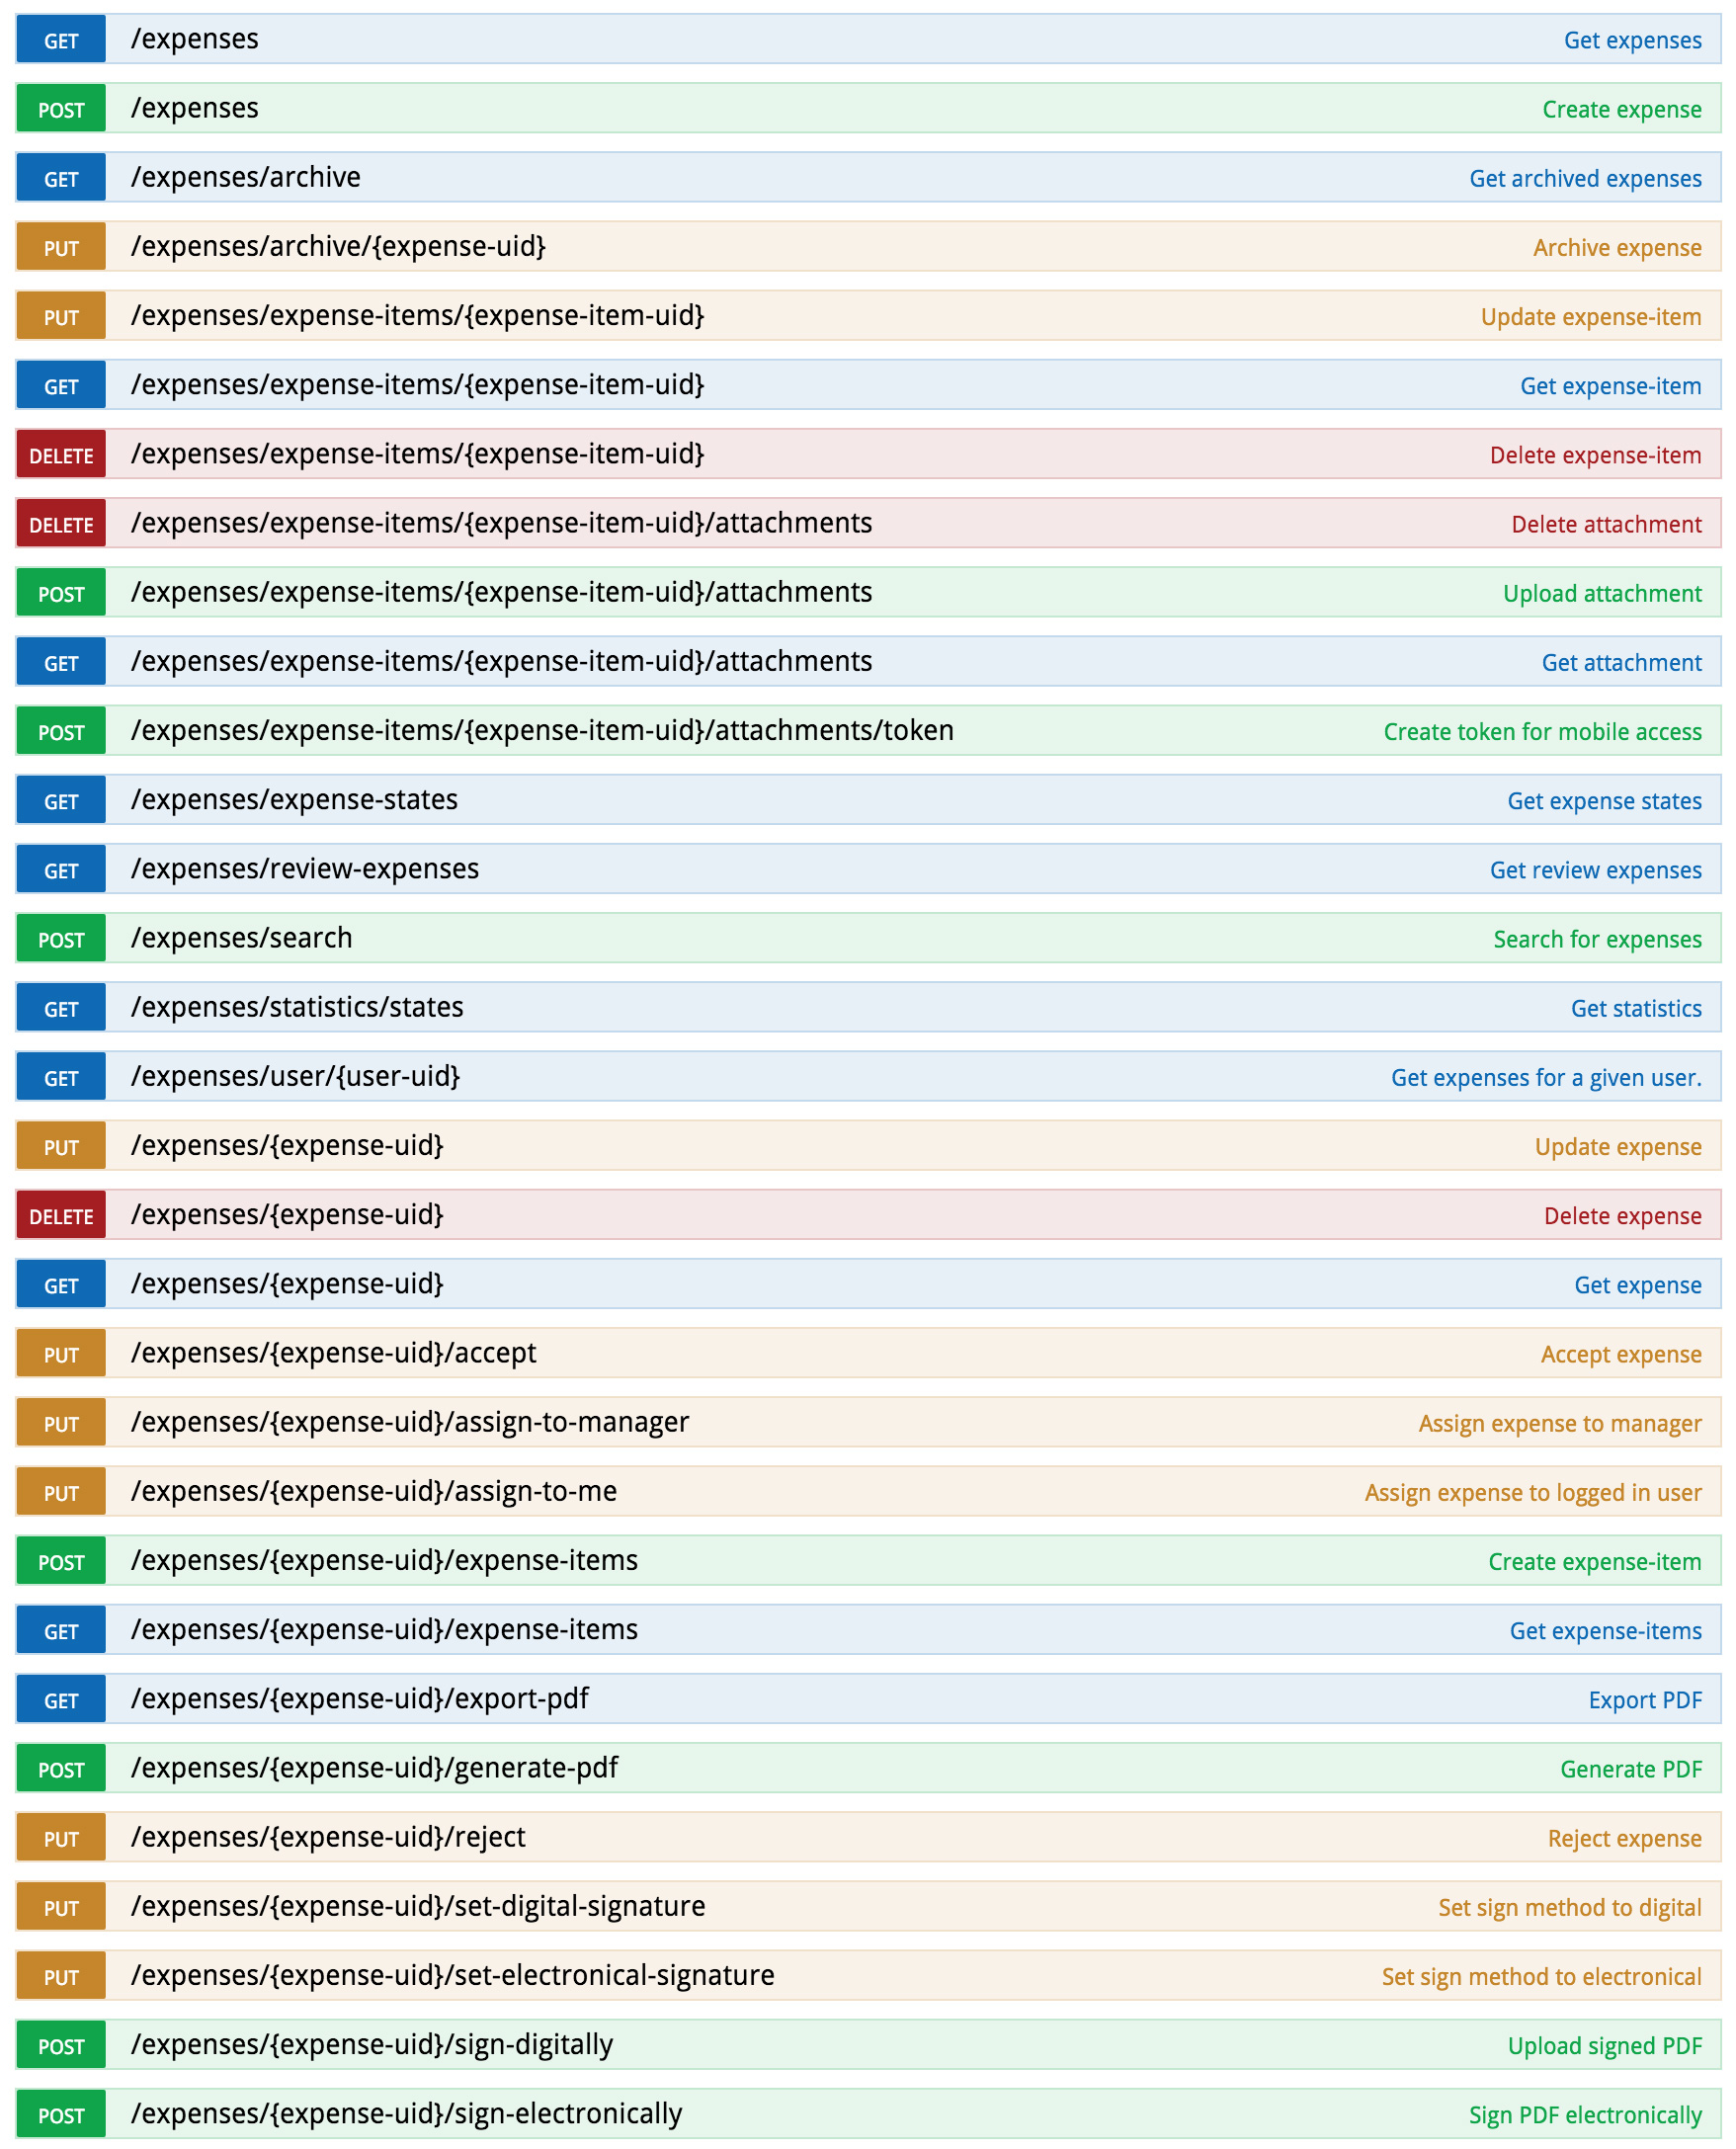
\includegraphics[width=0.95\textwidth]{rest-services_expense}}
\end{figure}
\newpage

\subsection{PRIVATE: finance administrator services}
\begin{figure}[H]
	{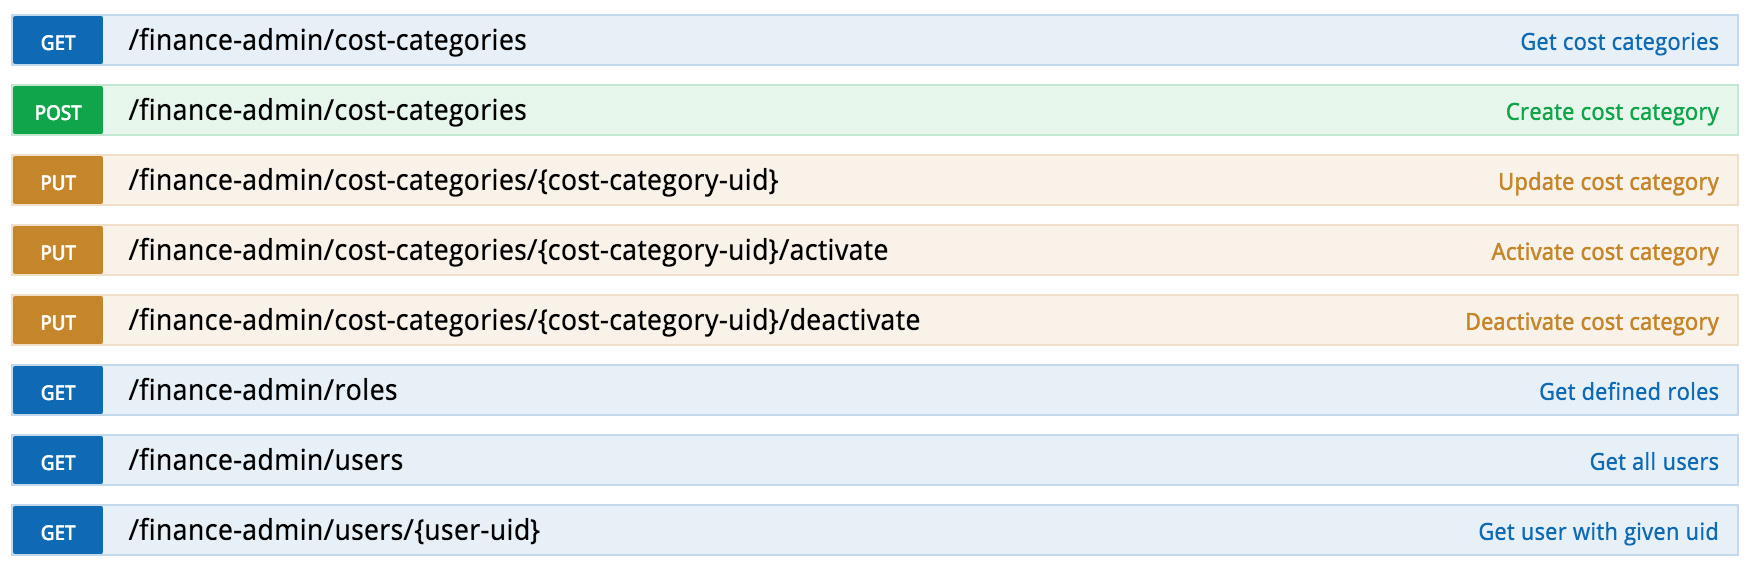
\includegraphics[width=0.95\textwidth]{rest-services_fa}}
\end{figure}

\subsection{PRIVATE: user services}
\begin{figure}[H]
	{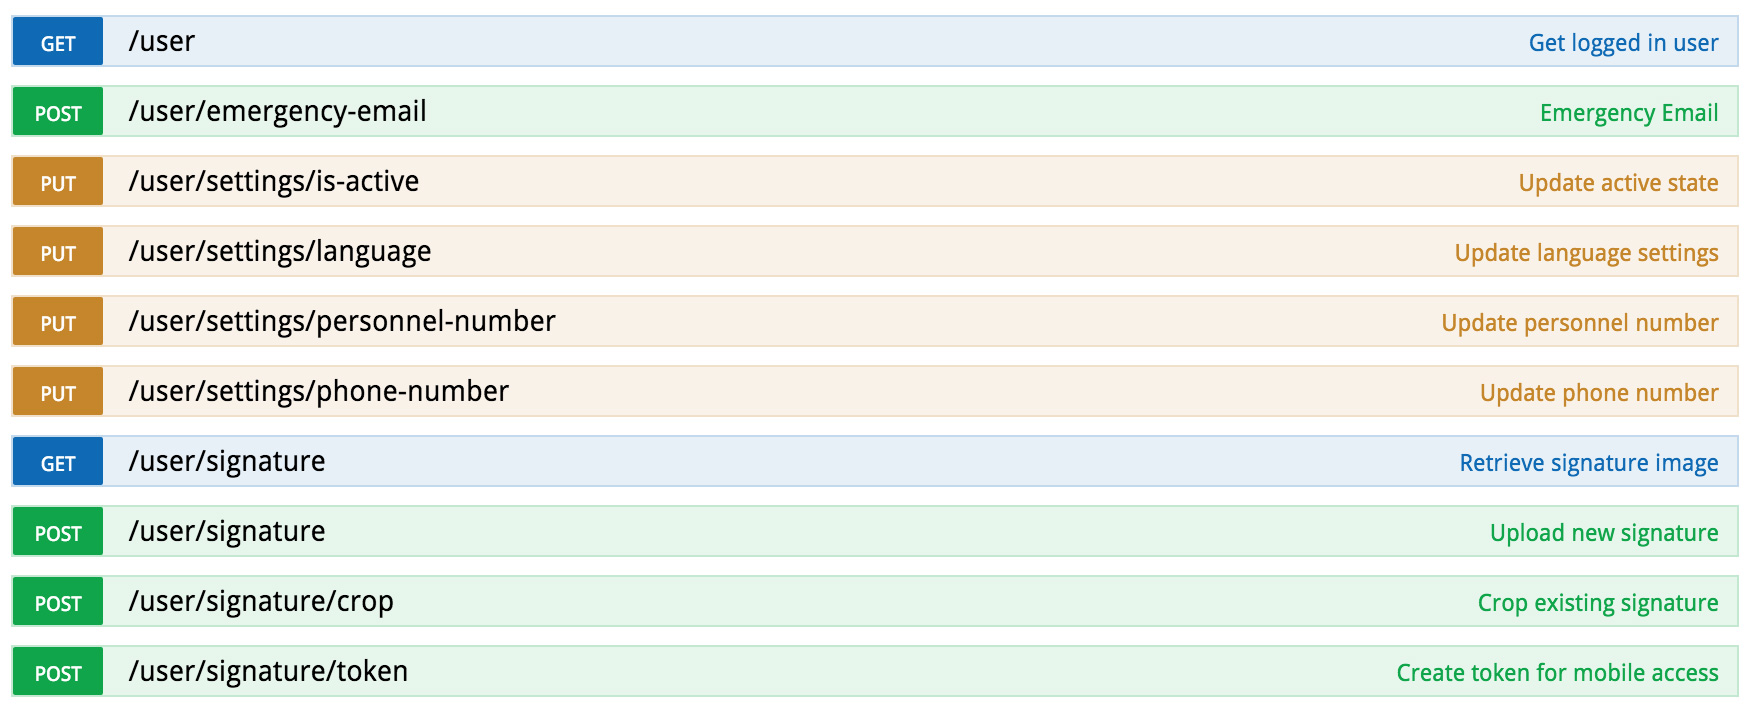
\includegraphics[width=0.95\textwidth]{rest-services_user}}
\end{figure}

\subsection{PUBLIC: various services}
\begin{figure}[H]
	{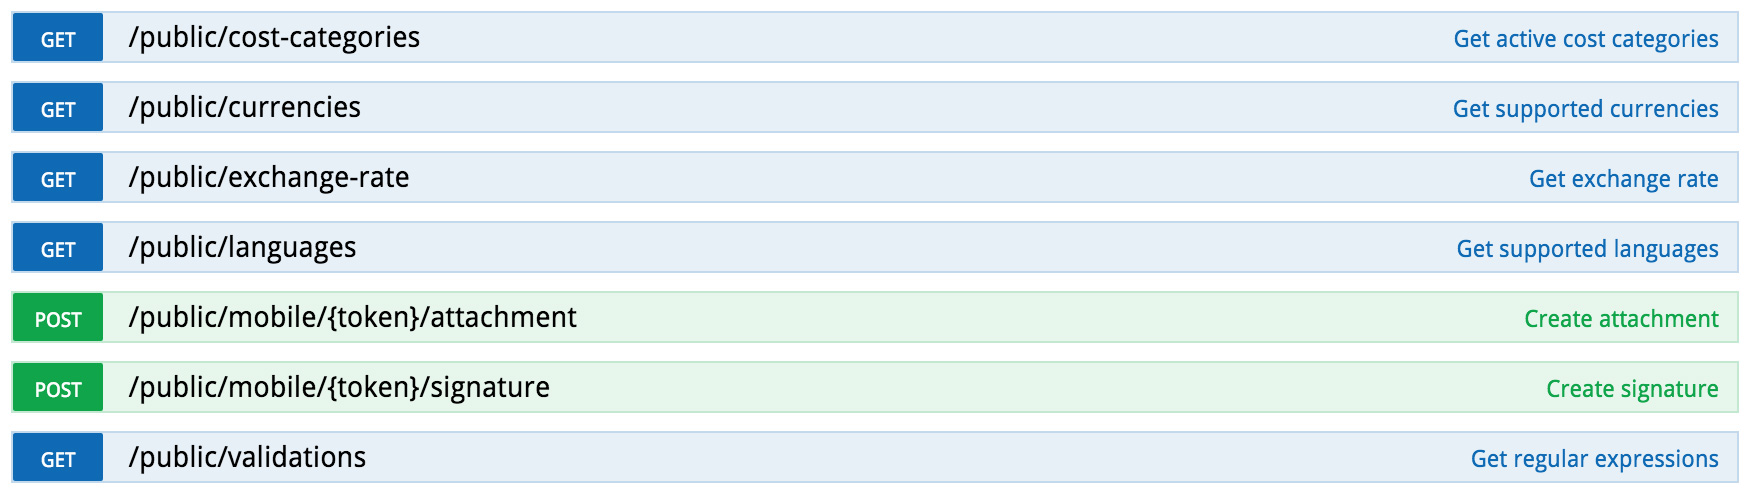
\includegraphics[width=0.95\textwidth]{rest-services_public}}
\end{figure}
\newpage

\section{PDF}
\label{sec:app-pdf}

\begin{figure}[H]
	{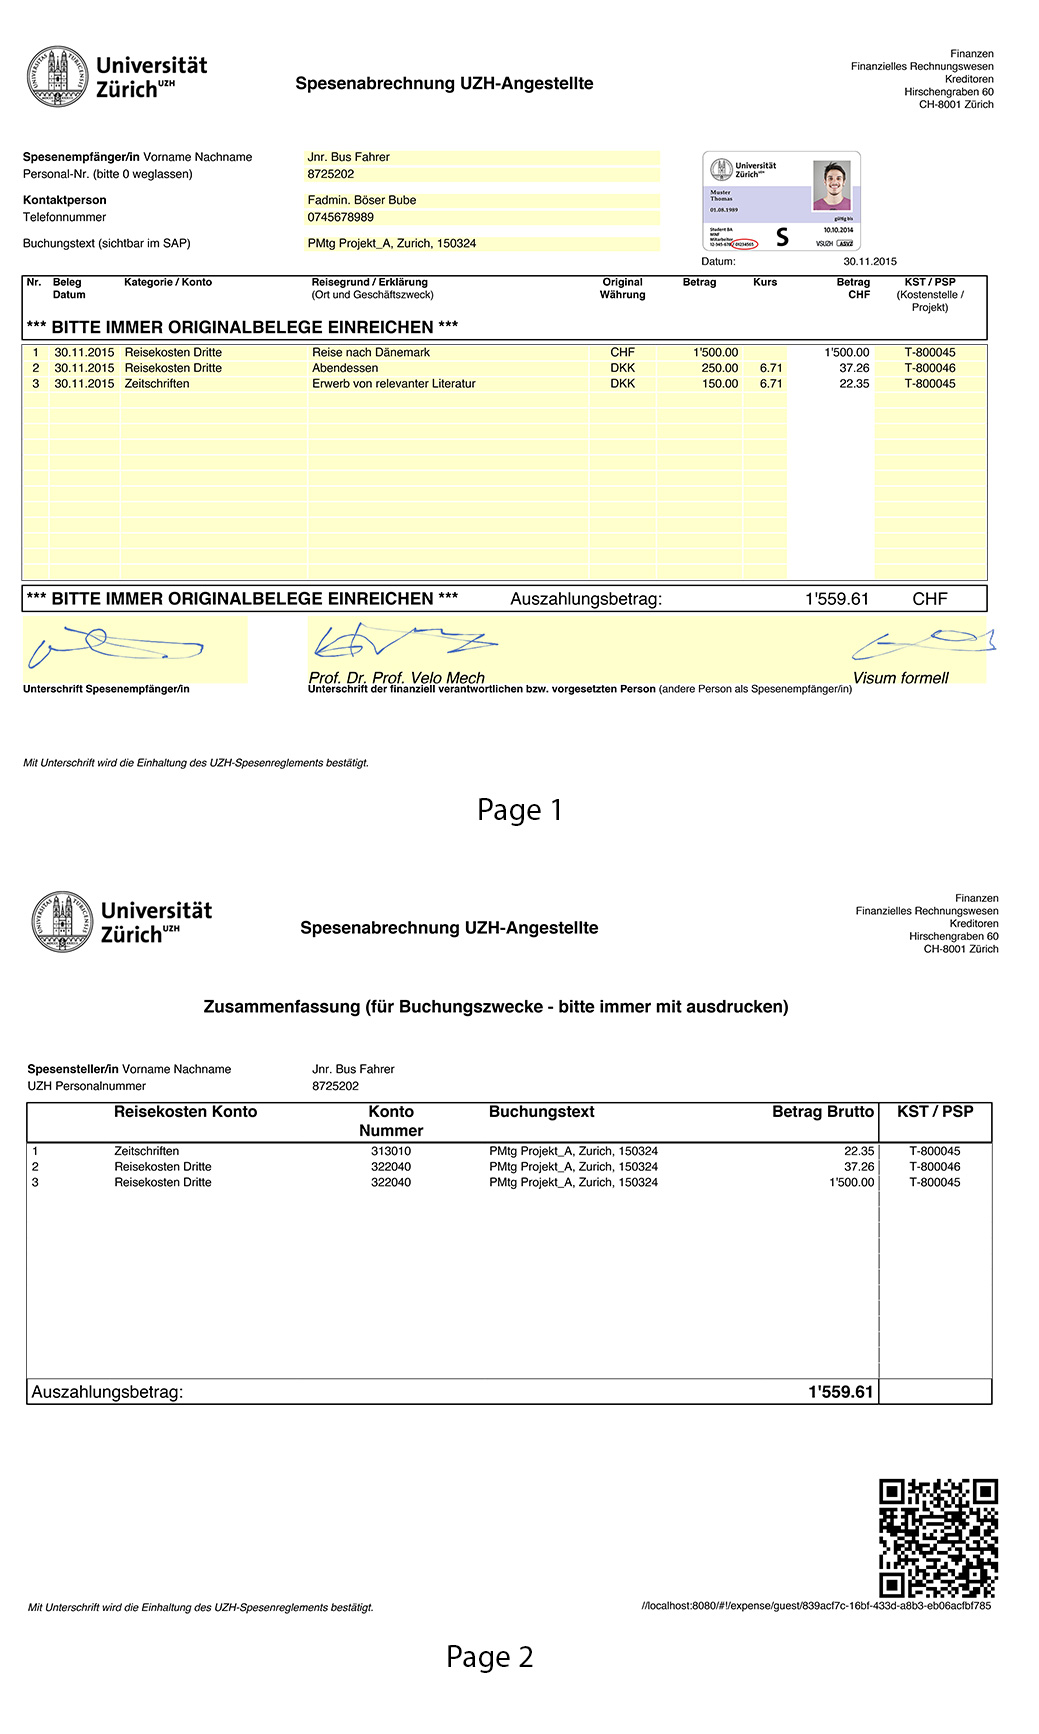
\includegraphics[width=0.8\textwidth]{pdf}}
\end{figure}
\newpage

\chapter{Reimbursement source-code}
\label{github-source}

The complete source code is available on a public repository on \url{http://github.com}. There exist four repositories: one for the front-end, one for the back-end, one for the technical documentation and one for the user manual.

\begin{itemize}
	\item Back-end: \newline \url{https://github.com/Communication-Systems-Group/reimbursement-server.git}
	\item Front-end: \newline \url{https://github.com/Communication-Systems-Group/reimbursement-client.git}
	\item Documentation: \newline \url{https://github.com/Communication-Systems-Group/reimbursement-documentation.git}
	\item User Manual: \newline \url{https://github.com/Communication-Systems-Group/reimbursement-manual.git}
\end{itemize}

For detailed installation instructions of the development environment and deployment steps, please refer to the developer guide \ref{chap:installation}.
